\chapter{L'énergie des réactions~: combustion et énergies de liaison}\label{ch:g11:reaction-energy}

On brise l'opercule d'une chaufferette et, une minute plus tard, elle
est trop chaude pour être tenue longtemps~; on presse une poche de froid
instantané et elle refroidit une cheville foulée~; un bus de ville roule
toute la journée au dihydrogène et ne laisse derrière lui que de la
vapeur d'eau. Les \omterm{def:g5:irreversible-changes:chemical-change}{transformations chimiques} ne changent pas seulement
des substances en d'autres~: elles libèrent de l'énergie, ou en
absorbent. D'où vient cette énergie, et combien un \omterm{def:g4:what-a-fire-needs:fuel}{combustible} peut-il
en fournir~?

\begin{recall}
Lors d'une \omterm{def:g8:combustion-and-fuels:complete}{combustion complète}, un \omterm{def:g4:what-a-fire-needs:fuel}{combustible} formé de carbone et
d'hydrogène \omterm{def:g4:what-a-fire-needs:burning}{brûle} dans le dioxygène en donnant du dioxyde de carbone et
de l'eau (\cref{ch:g8:combustion-and-fuels}). Une \omterm{def:g10:lewis-and-shape:covalent-bond}{liaison covalente} est
un doublet d'\omterm{def:g9:inside-the-atom:nucleus}{électrons} mis en commun~; le \omterm{def:g10:lewis-and-shape:lewis-structure}{schéma de Lewis} d'une \omterm{def:g7:atoms-and-molecules:molecule}{molécule}
montre toutes ses liaisons (\cref{ch:g10:lewis-and-shape}). La \omterm{def:g10:the-mole:amount}{quantité
de matière} se compte en \omterm{def:g10:the-mole:amount}{moles} (\cref{ch:g10:the-mole}).
\end{recall}

\begin{omfigure}
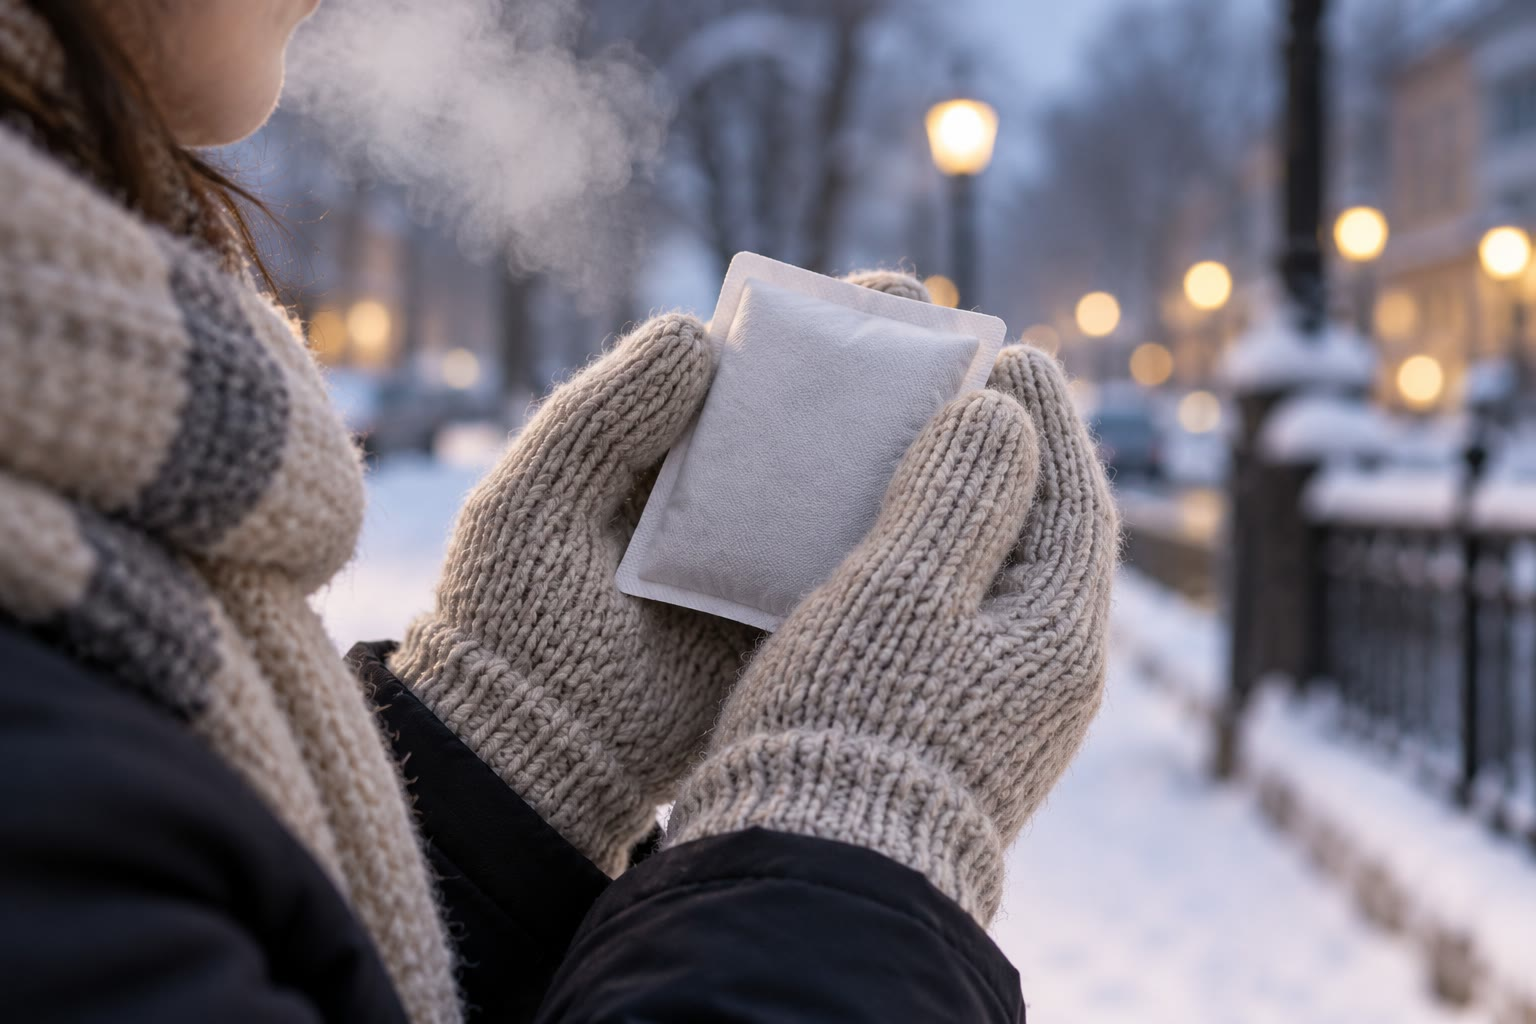
\includegraphics[width=0.45\linewidth]{images/book1/ai/g11-hand-warmers.jpg}

{\small Une chaufferette~: une réaction, à l'intérieur de la poche,
libère de la chaleur.}
\end{omfigure}

\section{Transformations exothermiques et endothermiques}

\begin{definition}[Exothermique, endothermique]\label{def:g11:reaction-energy:exothermic}
Une transformation est \emph{exothermique}\index{exothermique} si elle
cède de l'énergie au milieu extérieur, le plus souvent sous forme de
chaleur~: le milieu extérieur se réchauffe. Elle est
\emph{endothermique}\index{endothermique} si elle reçoit de l'énergie du
milieu extérieur~: celui-ci se refroidit, ou bien il faut chauffer pour
que la transformation se poursuive.
\end{definition}

\begin{example}[Chaud et froid]\label{ex:g11:reaction-energy:packs}
Les \omterm{def:g4:what-a-fire-needs:burning}{combustions} sont \omterm{def:g11:reaction-energy:exothermic}{exothermiques}, tout comme la lente réaction de la
poudre de fer avec le dioxygène de l'\omterm{def:g4:air-a-mixture-of-gases:air}{air} dans une chaufferette. La
dissolution du nitrate d'ammonium dans l'eau, utilisée dans les poches
de froid, est \omterm{def:g11:reaction-energy:exothermic}{endothermique}~; la décomposition du calcaire en chaux vive
et dioxyde de carbone l'est aussi, et elle n'a lieu que dans un four
très chaud.
\end{example}

\begin{omfigure}
\begin{tikzpicture}[font=\small]
  \begin{scope}
    \draw[->] (0,0) -- (0,3.2) node[above] {énergie};
    \draw[very thick, omDef] (0.5,2.5) -- (2.3,2.5) node[right, text=black] {réactifs};
    \draw[very thick, omProp] (0.5,0.8) -- (2.3,0.8) node[right, text=black] {produits};
    \draw[->, thick, omThm] (1.4,2.45) -- (1.4,0.85);
    \node[omThm, anchor=west, align=left] at (1.5,1.65) {énergie\\ libérée};
    \node[anchor=north] at (1.6,-0.15) {\textbf{exothermique}};
  \end{scope}
  \begin{scope}[xshift=6cm]
    \draw[->] (0,0) -- (0,3.2) node[above] {énergie};
    \draw[very thick, omDef] (0.5,0.8) -- (2.3,0.8) node[right, text=black] {réactifs};
    \draw[very thick, omProp] (0.5,2.5) -- (2.3,2.5) node[right, text=black] {produits};
    \draw[->, thick, omDef] (1.4,0.85) -- (1.4,2.45);
    \node[omDef, anchor=west, align=left] at (1.5,1.65) {énergie\\ reçue};
    \node[anchor=north] at (1.6,-0.15) {\textbf{endothermique}};
  \end{scope}
\end{tikzpicture}

{\small Diagrammes énergétiques. Dans une réaction \omterm{def:g11:reaction-energy:exothermic}{exothermique}, les
produits possèdent moins d'énergie que les \omterm{def:g7:chemical-reactions:reactant}{réactifs}, et la différence
est libérée~; dans une réaction \omterm{def:g11:reaction-energy:exothermic}{endothermique}, ils en possèdent plus, et
il faut la fournir.}
\end{omfigure}

\section{L'énergie libérée par une combustion}

\begin{definition}[Énergie molaire de combustion]\label{def:g11:reaction-energy:combustion-energy}
L'\emph{énergie molaire de combustion}\index{energie molaire de combustion@énergie molaire de combustion}
$E_c$ d'un \omterm{def:g4:what-a-fire-needs:fuel}{combustible} est l'énergie libérée par la \omterm{def:g8:combustion-and-fuels:complete}{combustion complète}
d'une \omterm{def:g10:the-mole:amount}{mole} de ce \omterm{def:g4:what-a-fire-needs:fuel}{combustible}, en \si{kJ/mol}, l'eau formée étant
liquide.
\end{definition}

\begin{proposition}[Énergie libérée par $n$ moles]\label{prop:g11:reaction-energy:n-moles}
% ledger: dch:CH4
La \omterm{def:g8:combustion-and-fuels:complete}{combustion complète} d'une quantité $n$ de \omterm{def:g4:what-a-fire-needs:fuel}{combustible} libère
l'énergie $Q = n \times E_c$. Pour le méthane,
$E_c = \qty{890.7}{kJ/mol}$~: la \omterm{def:g4:what-a-fire-needs:burning}{combustion} de \qty{1.00}{mol}
(\qty{16.0}{g}) de méthane libère environ \qty{891}{kJ}.
\end{proposition}

\begin{proof}
Chaque \omterm{def:g10:the-mole:amount}{mole} de \omterm{def:g4:what-a-fire-needs:fuel}{combustible} brûlée libère $E_c$~; $n$ \omterm{def:g10:the-mole:amount}{moles} libèrent
$n$ fois plus.
\end{proof}

\begin{inthelab}[Chauffer de l'eau avec une lampe à alcool]
% ledger: cp:water
On pèse une lampe à \omterm{def:g11:functional-groups:alcohol}{alcool} remplie d'éthanol, puis on l'allume sous une
canette métallique contenant \qty{200}{g} d'eau, dans laquelle plonge un
thermomètre. Quand l'eau s'est réchauffée de \qty{25}{\celsius}, on
éteint la flamme et on pèse de nouveau la lampe~: elle a perdu
\qty{1.50}{g} d'éthanol. L'énergie reçue par l'eau se calcule avec la
formule de physique $Q = m\, c\, \Delta\theta$,
où $c = \qty{4.18}{J/(g.\celsius)}$ est la capacité thermique massique
de l'eau. Elle est bien inférieure à l'énergie que l'éthanol pourrait
libérer~: une grande partie de la chaleur réchauffe l'\omterm{def:g4:air-a-mixture-of-gases:air}{air}, la canette et
la lampe, et une partie de l'éthanol \omterm{def:g4:what-a-fire-needs:burning}{brûle} de façon incomplète.
\end{inthelab}

\begin{omfigure}
\begin{tikzpicture}[font=\small]
  % spirit burner
  \fill[black!8, draw=black!60] (-0.6,0) rectangle (0.6,0.7);
  \fill[cyan!15] (-0.55,0.05) rectangle (0.55,0.45);
  \fill[black!40] (-0.06,0.7) rectangle (0.06,0.95);
  \fill[orange!70!yellow] (0,0.95) .. controls (-0.25,1.25) and (-0.1,1.6) .. (0,1.85)
    .. controls (0.1,1.6) and (0.25,1.25) .. (0,0.95);
  \fill[yellow!40] (0,1.0) .. controls (-0.1,1.2) and (-0.05,1.4) .. (0,1.5)
    .. controls (0.05,1.4) and (0.1,1.2) .. (0,1.0);
  % tripod and can
  \draw[black!60, line width=1pt] (-1.1,0) -- (-0.9,2.1) (1.1,0) -- (0.9,2.1);
  \draw[black!60, line width=1.2pt] (-1.1,2.1) -- (1.1,2.1);
  \fill[black!15, draw=black!60] (-0.8,2.1) rectangle (0.8,3.7);
  \fill[omWater] (-0.75,2.15) rectangle (0.75,3.3);
  % thermometer
  \pic at (0.35,2.35) {thermometer};
  \draw[omProp, thick, <-] (0.6,0.35) -- (2.0,0.35) node[right, text=black]
    {lampe à alcool (éthanol)};
  \draw[omProp, thick, <-] (0.8,2.9) -- (2.0,2.9) node[right, text=black]
    {canette~: \qty{200}{g} d'eau};
  \draw[omProp, thick, <-] (0.45,5.0) -- (2.0,5.0) node[right, text=black]
    {thermomètre};
\end{tikzpicture}

{\small Mesurer l'énergie fournie par un \omterm{def:g4:what-a-fire-needs:fuel}{combustible}~: une lampe à
\omterm{def:g11:functional-groups:alcohol}{alcool} chauffe une canette d'eau dont on mesure l'élévation de
température.}
\end{omfigure}


\begin{example}[La lampe à alcool en chiffres]\label{ex:g11:reaction-energy:burner}
% ledger: cp:water, dch:C2H5OH, aw:C, aw:H, aw:O
L'eau a reçu $Q = 200 \times 4.18 \times 25 = \qty{2.09e4}{J}$,
soit \qty{20.9}{kJ}. L'éthanol brûlé, \qty{1.50}{g}, représente
$1.50 / 46.0 = \qty{0.0326}{mol}$~; avec $E_c = \qty{1367.6}{kJ/mol}$, il
pourrait libérer $0.0326 \times 1367.6 = \qty{44.6}{kJ}$. Seuls
$20.9 / 44.6 \approx \qty{47}{\percent}$ de cette énergie ont atteint
l'eau.
\end{example}

\section{Les énergies de liaison}

\begin{definition}[Énergie de liaison]\label{def:g11:reaction-energy:bond-energy}
L'\emph{énergie de liaison}\index{energie de liaison@énergie de liaison} d'une \omterm{def:g10:lewis-and-shape:covalent-bond}{liaison
covalente} est l'énergie nécessaire pour rompre une \omterm{def:g10:the-mole:amount}{mole} de telles
liaisons, les \omterm{def:g7:atoms-and-molecules:molecule}{molécules} et les \omterm{def:g7:atoms-and-molecules:atom}{atomes} étant à l'état gazeux. Les tables
donnent des valeurs moyennes, mesurées sur de nombreuses \omterm{def:g7:atoms-and-molecules:molecule}{molécules}, en
\si{kJ/mol}.
\end{definition}

\begin{omfigure}
\small
% ledger: be:H-H, be:C-H, be:N-H, be:O-H, be:H-Cl, be:C-C, be:CC-double, be:C-O, be:CO-double, be:NN-triple, be:OO-double, be:Cl-Cl
\begin{tabular}{lr@{\qquad}lr@{\qquad}lr}
\hline
liaison & \si{kJ/mol} & liaison & \si{kJ/mol} & liaison & \si{kJ/mol} \\
\hline
\ce{H-H} & 436 & \ce{C-C} & 345 & \ce{O=O} & 498 \\
\ce{C-H} & 415 & \ce{C=C} & 611 & \ce{N#N} & 946 \\
\ce{N-H} & 390 & \ce{C-O} & 350 & \ce{Cl-Cl} & 243 \\
\ce{O-H} & 464 & \ce{C=O} & 741 & \ce{H-Cl} & 432 \\
\hline
\end{tabular}\par\medskip

{\small \omterm{def:g11:reaction-energy:bond-energy}{Énergies de liaison} moyennes. Rompre une liaison coûte toujours
de l'énergie~; la former restitue la même énergie.}
\end{omfigure}

\begin{omfigure}
\begin{tikzpicture}[font=\small, x=1cm, y=0.0015cm]
  \draw[->] (0,-850) -- (0,2900) node[above] {énergie (\si{kJ})};
  \draw[very thick, black!60] (0.4,2656) -- (3.9,2656);
  \node[anchor=west] at (4.0,2656) {atomes séparés~: \ce{C + 4H + 4O}};
  \draw[very thick, omDef] (0.4,0) -- (3.9,0);
  \node[anchor=west] at (4.0,0) {\ce{CH4 + 2O2}};
  \draw[very thick, omProp] (0.4,-682) -- (3.9,-682);
  \node[anchor=west] at (4.0,-682) {\ce{CO2 + 2H2O}};
  \draw[->, thick, omDef] (1.0,30) -- (1.0,2626);
  \node[omDef, anchor=west, align=left] at (1.05,1500) {rompre\\ 4 \ce{C-H} et\\ 2 \ce{O=O}~:\\ $+\qty{2656}{kJ}$};
  \draw[->, thick, omProp] (3.4,2626) -- (3.4,-652);
  \node[omProp, anchor=west, align=left] at (3.45,1200) {former 2 \ce{C=O}\\ et 4 \ce{O-H}~:\\ $-\qty{3338}{kJ}$};
  \draw[<->, omThm, thick] (0.6,-10) -- (0.6,-672);
  \node[omThm, anchor=west] at (0.65,-341) {$E_r \approx \qty{-682}{kJ}$};
\end{tikzpicture}

{\small La \omterm{def:g4:what-a-fire-needs:burning}{combustion} du méthane décomposée en deux étapes imaginaires,
avec les \omterm{def:g11:reaction-energy:bond-energy}{énergies de liaison} moyennes~: rupture de toutes les liaisons,
puis formation des nouvelles. L'estimation, \qty{-682}{kJ} par \omterm{def:g10:the-mole:amount}{mole} de
méthane, correspond à une réaction \omterm{def:g11:reaction-energy:exothermic}{exothermique}.}
\end{omfigure}

\begin{proposition}[Estimer une énergie de réaction]\label{prop:g11:reaction-energy:estimate}
Pour une réaction entre gaz, l'énergie reçue, $E_r$ (négative si de
l'énergie est libérée), vaut approximativement
\[
  E_r \approx \sum E(\text{liaisons rompues}) - \sum E(\text{liaisons formées}) .
\]
Si $E_r < 0$, la formation des nouvelles liaisons libère plus d'énergie
qu'il n'en faut pour rompre les anciennes~: la réaction est
\omterm{def:g11:reaction-energy:exothermic}{exothermique}.
\end{proposition}

\begin{proof}
On imagine la réaction en deux étapes~: toutes les liaisons des \omterm{def:g7:chemical-reactions:reactant}{réactifs}
sont rompues, ce qui coûte la première somme et laisse des \omterm{def:g7:atoms-and-molecules:atom}{atomes}
séparés~; puis les liaisons des produits se forment, ce qui restitue la
seconde somme. Le résultat n'est qu'une estimation, car les tables
donnent des moyennes sur de nombreuses \omterm{def:g7:atoms-and-molecules:molecule}{molécules}.
\end{proof}

\begin{method}[Estimer une énergie de réaction à partir des énergies de liaison]\label{met:g11:reaction-energy:bonds}
\begin{enumerate}
  \item Écrire l'\omterm{def:g8:balanced-equations:equation}{équation ajustée} et le \omterm{def:g10:lewis-and-shape:lewis-structure}{schéma de Lewis} de chaque
        \omterm{def:g7:atoms-and-molecules:molecule}{molécule}.
  \item Compter les liaisons de chaque type rompues dans les \omterm{def:g7:chemical-reactions:reactant}{réactifs} et
        formées dans les produits, en tenant compte des coefficients.
  \item Additionner les \omterm{def:g11:reaction-energy:bond-energy}{énergies des liaisons} rompues, puis soustraire
        celles des liaisons formées.
  \item Conclure~: un résultat négatif signifie une réaction
        \omterm{def:g11:reaction-energy:exothermic}{exothermique}.
\end{enumerate}
\end{method}

\begin{example}[Le dihydrogène et le dichlore]\label{ex:g11:reaction-energy:hcl}
% ledger: be:H-H, be:Cl-Cl, be:H-Cl
Pour \ce{H2 + Cl2 -> 2HCl}~: une liaison \ce{H-H} et une \ce{Cl-Cl}
rompues, $436 + 243 = \qty{679}{kJ}$~; deux \ce{H-Cl} formées, $2 \times 432 =
\qty{864}{kJ}$. Donc $E_r \approx 679 - 864 = \qty{-185}{kJ}$ par \omterm{def:g10:the-mole:amount}{mole}
de réaction~: la réaction est \omterm{def:g11:reaction-energy:exothermic}{exothermique}.
\end{example}


\begin{remark}[Estimation et mesure]\label{rem:g11:reaction-energy:compare}
% ledger: dch:CH4
L'énergie mesurée libérée par la \omterm{def:g4:what-a-fire-needs:burning}{combustion} d'une \omterm{def:g10:the-mole:amount}{mole} de méthane vaut
\qty{890.7}{kJ}, plus que l'estimation. Il y a trois raisons à cela~:
les liaisons \ce{C=O} du dioxyde de carbone sont plus fortes que la
liaison \ce{C=O} moyenne de la table~; la valeur mesurée correspond à
de l'eau liquide, et la condensation de la vapeur d'eau libère encore de
l'énergie~; enfin, les \omterm{def:g11:reaction-energy:bond-energy}{énergies de liaison} moyennes ne sont que des
moyennes. La méthode des \omterm{def:g11:reaction-energy:bond-energy}{énergies de liaison} donne le signe et l'ordre
de grandeur, pas la valeur exacte.
\end{remark}

\section{Comparer les combustibles}

\begin{omfigure}
\begin{tikzpicture}
\begin{axis}[xbar, width=0.78\linewidth, height=5.4cm, xmin=0, xmax=160,
    xlabel={énergie libérée par kilogramme brûlé (\si{MJ/kg})},
    symbolic y coords={ethanol, octane, propane, methane, hydrogen},
    yticklabels={éthanol, octane, propane, méthane, dihydrogène},
    ytick=data, bar width=10pt, nodes near coords,
    nodes near coords style={font=\footnotesize, /pgf/number format/fixed,
      /pgf/number format/precision=1, /pgf/number format/fixed zerofill},
    tick label style={font=\small}, label style={font=\small},
    axis lines*=left, xmajorgrids, grid style={gray!20}, enlarge y limits=0.15]
  % ledger: dch:C2H5OH, dfh:C8H18, dfh:CO2, dfh:H2O-l, dch:C3H8, dch:CH4 (per kg with the book's molar masses)
  \addplot[fill=omProp!55, draw=omProp] coordinates {(29.7,ethanol) (48.0,octane)
    (50.4,propane) (55.7,methane) (142.9,hydrogen)};
\end{axis}
\end{tikzpicture}

{\small Énergie libérée par la \omterm{def:g8:combustion-and-fuels:complete}{combustion complète} d'un kilogramme de
cinq \omterm{def:g4:what-a-fire-needs:fuel}{combustibles} (eau formée à l'état liquide). Le dihydrogène fournit
de loin le plus d'énergie par kilogramme~; l'éthanol, déjà en partie
«~brûlé~» (il contient de l'oxygène), le moins.}
\end{omfigure}

\begin{example}[Le dioxyde de carbone par mégajoule]\label{ex:g11:reaction-energy:co2}
% ledger: dch:CH4, dch:C2H5OH
La \omterm{def:g4:what-a-fire-needs:burning}{combustion} d'une \omterm{def:g10:the-mole:amount}{mole} de méthane libère \qty{890.7}{kJ} et une \omterm{def:g10:the-mole:amount}{mole}
de dioxyde de carbone, soit \qty{44.0}{g}. Pour un mégajoule,
\qty{1000}{kJ}, elle libère donc
$44.0 \times 1000 / 890.7 = \qty{49.4}{g}$ de dioxyde de carbone.
L'éthanol, avec deux \omterm{def:g10:the-mole:amount}{moles} de dioxyde de carbone pour \qty{1367.6}{kJ},
en libère $88.0 \times 1000 / 1367.6 = \qty{64.3}{g}$ par mégajoule. Le
dihydrogène n'en libère pas du tout~: son seul produit est l'eau.
\end{example}

\begin{omfigure}
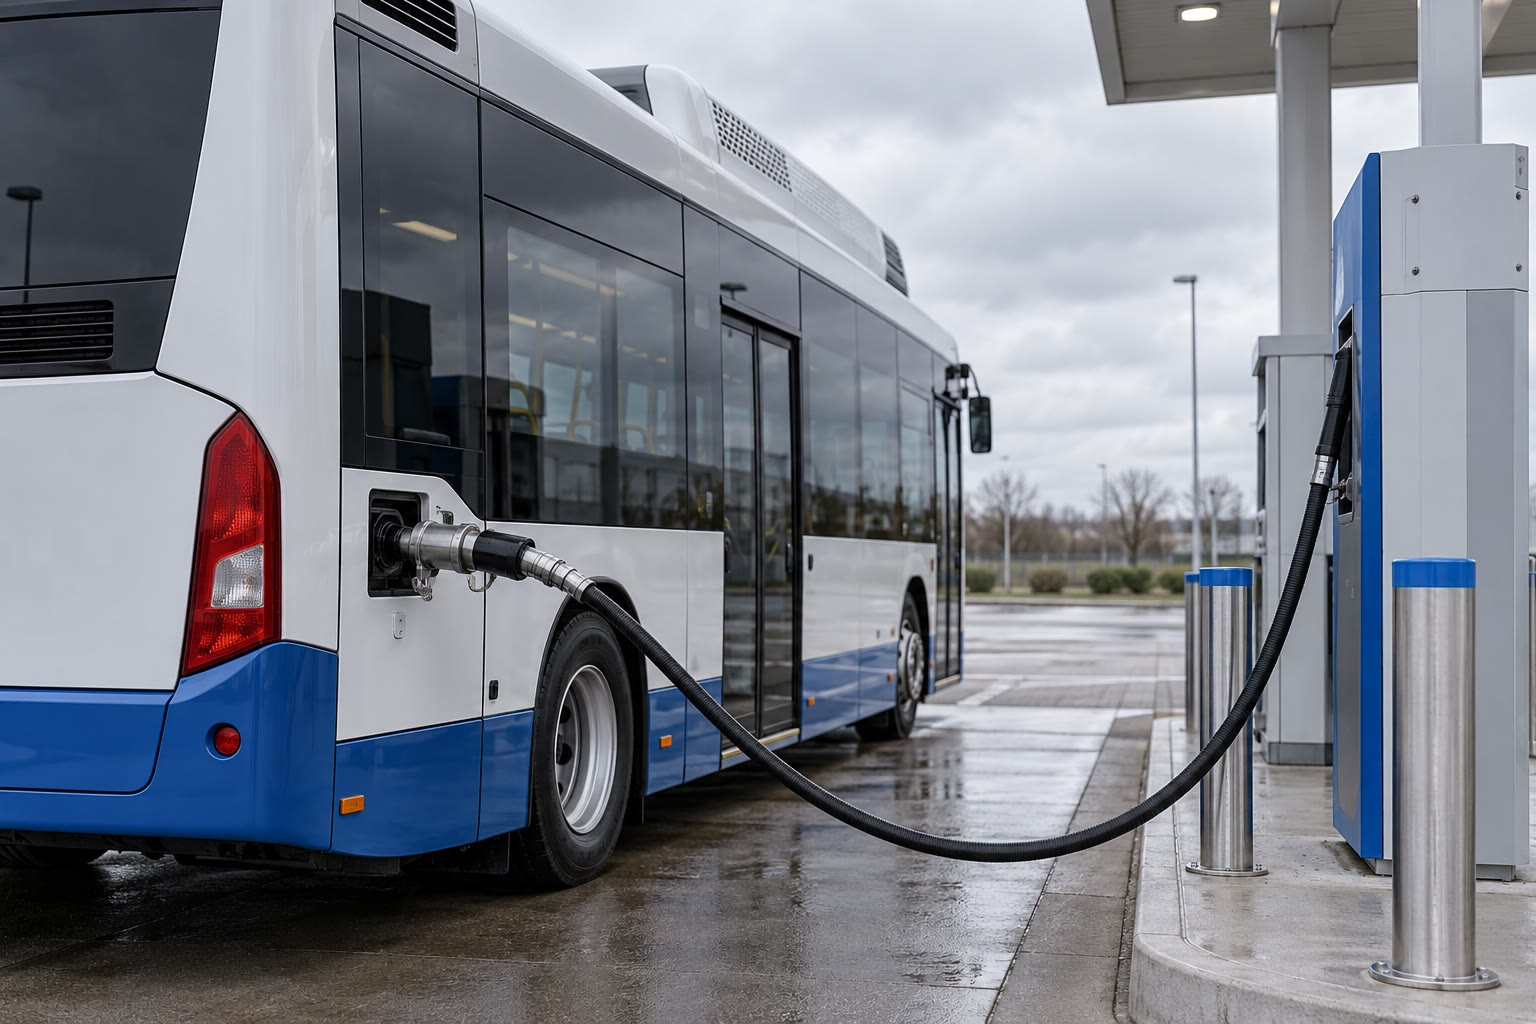
\includegraphics[width=0.5\linewidth]{images/book1/ai/g11-hydrogen-bus.jpg}

{\small Un bus dans une station de dihydrogène~: son \omterm{def:g4:what-a-fire-needs:fuel}{combustible} ne
rejette que de l'eau.}
\end{omfigure}

\begin{safety}{\ghs[0.82cm]{GHS02}\ghs[0.82cm]{GHS07}}
% ledger: ghs:ethanol
L'éthanol est très inflammable et irritant pour les yeux. Une lampe à
\omterm{def:g11:functional-groups:alcohol}{alcool} se remplit loin de toute flamme, ne se remplit jamais à chaud, et
n'est utilisée que par le professeur, sur un support résistant à la
chaleur.
\end{safety}

\section{Exercices}


\begin{exercise}[$\star$]\label{exo:g11:reaction-energy:1}
\omterm{def:g11:reaction-energy:exothermic}{Exothermique} ou \omterm{def:g11:reaction-energy:exothermic}{endothermique}~: du bois qui \omterm{def:g4:what-a-fire-needs:burning}{brûle}~; de la glace qui
fond~; une poche de froid que l'on presse~; une chaufferette qui
chauffe~; une feuille verte qui fabrique du sucre à la lumière du
soleil~?
\end{exercise}

\begin{exercise}[$\star$]\label{exo:g11:reaction-energy:2}
% ledger: dch:CH4
Quelle énergie la \omterm{def:g8:combustion-and-fuels:complete}{combustion complète} de \qty{3.0}{mol} de méthane
libère-t-elle~?
\end{exercise}

\begin{exercise}[$\star$]\label{exo:g11:reaction-energy:3}
Sur le diagramme énergétique d'une réaction \omterm{def:g11:reaction-energy:exothermic}{exothermique}, qui possède le
plus d'énergie, les \omterm{def:g7:chemical-reactions:reactant}{réactifs} ou les produits~? Où va la différence~?
\end{exercise}

\begin{exercise}[$\star$]\label{exo:g11:reaction-energy:4}
% ledger: dch:C2H5OH
Quelle énergie la \omterm{def:g8:combustion-and-fuels:complete}{combustion complète} de \qty{100}{g} d'éthanol
libère-t-elle~?
\end{exercise}

\begin{exercise}[$\star$]\label{exo:g11:reaction-energy:5}
Qu'est-ce qu'une \omterm{def:g11:reaction-energy:bond-energy}{énergie de liaison}~? Pourquoi rompre une liaison
coûte-t-il toujours de l'énergie~?
\end{exercise}

\begin{exercise}[$\star\star$]\label{exo:g11:reaction-energy:6}
Estimer, à l'aide des \omterm{def:g11:reaction-energy:bond-energy}{énergies de liaison}, l'énergie de la réaction
\ce{2H2 + O2 -> 2H2O}, toutes les espèces étant gazeuses. Est-elle
\omterm{def:g11:reaction-energy:exothermic}{exothermique}~?
\end{exercise}

\begin{exercise}[$\star\star$]\label{exo:g11:reaction-energy:7}
Estimer l'énergie de la \omterm{def:g4:what-a-fire-needs:burning}{combustion} de l'éthanol, \ce{C2H5OH + 3O2 ->
2CO2 + 3H2O}, à l'aide des \omterm{def:g11:reaction-energy:bond-energy}{énergies de liaison} (dessiner d'abord le
\omterm{def:g10:lewis-and-shape:lewis-structure}{schéma de Lewis} de l'éthanol), et comparer avec la valeur mesurée,
\qty{1367.6}{kJ/mol}.
\end{exercise}

\begin{exercise}[$\star\star$]\label{exo:g11:reaction-energy:8}
% ledger: dch:C3H8, dch:CH4
Calculer l'énergie libérée par kilogramme de propane
(\qty{2219.2}{kJ/mol}) et de méthane. Comparer avec le diagramme en
barres.
\end{exercise}

\begin{exercise}[$\star\star$]\label{exo:g11:reaction-energy:9}
% ledger: cp:water, dch:CH4
Une cuisinière à gaz chauffe \qty{1.50}{L} d'eau (\qty{1500}{g}) de
\qty{15}{\celsius} à \qty{100}{\celsius}. Quelle énergie l'eau
reçoit-elle~? Quelle masse de méthane brûle-t-on si toute l'énergie
atteint l'eau~? Si seule la moitié l'atteint~?
\end{exercise}

\begin{exercise}[$\star\star$]\label{exo:g11:reaction-energy:10}
À l'aide du diagramme en barres, classer les \omterm{def:g4:what-a-fire-needs:fuel}{combustibles} selon leur
énergie par kilogramme. Quelle masse de dihydrogène fournit la même
énergie que \qty{1.0}{kg} d'octane~?
\end{exercise}

\begin{exercise}[$\star\star$]\label{exo:g11:reaction-energy:11}
Estimer l'énergie de la réaction \ce{N2 + 3H2 -> 2NH3}, toutes les
espèces étant gazeuses. Est-elle \omterm{def:g11:reaction-energy:exothermic}{exothermique} ou \omterm{def:g11:reaction-energy:exothermic}{endothermique}~?
\end{exercise}

\begin{exercise}[$\star\star\star$]\label{exo:g11:reaction-energy:12}
% ledger: cp:water, dch:C2H5OH
Lors d'une expérience avec une lampe à \omterm{def:g11:functional-groups:alcohol}{alcool}, \qty{250}{g} d'eau se
réchauffent de \qty{20}{\celsius} pendant que \qty{1.20}{g} d'éthanol
brûlent. Calculer l'énergie reçue par l'eau, l'énergie que l'éthanol
pourrait libérer, et le rendement du chauffage. Citer trois causes de
pertes.
\end{exercise}

\begin{exercise}[$\star\star\star$]\label{exo:g11:reaction-energy:13}
% ledger: dfh:C8H18, dfh:CO2, dfh:H2O-l, dch:C3H8
L'octane libère \qty{5470}{kJ/mol} et le propane \qty{2219.2}{kJ/mol}.
Écrire leurs équations de \omterm{def:g4:what-a-fire-needs:burning}{combustion} et calculer la masse de dioxyde de
carbone que chacun libère par mégajoule. Comparer avec le méthane,
\qty{49.4}{g}.
\end{exercise}

\begin{exercise}[$\star\star\star$]\label{exo:g11:reaction-energy:14}
Pour le méthane comme pour l'éthanol, l'estimation par les \omterm{def:g11:reaction-energy:bond-energy}{énergies de
liaison} est inférieure à l'énergie libérée mesurée. En donner les
raisons, et expliquer pourquoi l'estimation reste utile.
\end{exercise}

\begin{exercise}[$\star\star\star$]\label{exo:g11:reaction-energy:15}
Estimer l'énergie de la réaction \ce{2H2O -> 2H2 + O2}, toutes les
espèces étant gazeuses. Pourquoi faut-il fournir de l'énergie (par
exemple sous forme électrique) pour produire du dihydrogène à partir de
l'eau~? Expliquer pourquoi on dit que le dihydrogène est un moyen de
\emph{stocker} l'énergie plutôt qu'une source d'énergie.
\end{exercise}

\section{Problème~: quel combustible pour le bus de la ville~?}

\begin{problem}[{Problème du week-end --- méthane, éthanol, octane ou
dihydrogène~: lequel fournit le plus d'énergie par kilogramme, et
combien de dioxyde de carbone par mégajoule~?}]
\label{pb:g11:reaction-energy:1}
% ledger: dch:CH4, dch:C2H5OH, dfh:C8H18, dfh:CO2, dfh:H2O-l, be:C-H, be:OO-double, be:CO-double, be:O-H
Une ville compare quatre \omterm{def:g4:what-a-fire-needs:fuel}{combustibles} pour ses bus~: le méthane (gaz
naturel), l'éthanol, l'octane (pour l'essence) et le dihydrogène. Les
énergies libérées par la \omterm{def:g8:combustion-and-fuels:complete}{combustion complète} d'une \omterm{def:g10:the-mole:amount}{mole} sont~: méthane
\qty{890.7}{kJ}, éthanol \qty{1367.6}{kJ}, octane \qty{5470}{kJ},
dihydrogène \qty{285.8}{kJ}, l'eau étant formée à l'état liquide.

\medskip
\noindent\textbf{Partie I --- Équations de \omterm{def:g4:what-a-fire-needs:burning}{combustion}.}
\begin{enumerate}
  \item Écrire l'équation de la \omterm{def:g8:combustion-and-fuels:complete}{combustion complète} du méthane.
  \item De l'éthanol, \ce{C2H6O}.
  \item De l'octane, \ce{C8H18}.
  \item Du dihydrogène.
  \item Quel \omterm{def:g4:what-a-fire-needs:fuel}{combustible} ne libère pas de dioxyde de carbone~?
\end{enumerate}

\medskip
\noindent\textbf{Partie II --- L'énergie par kilogramme.}
\begin{enumerate}[resume]
  \item Calculer les \omterm{def:g10:the-mole:molar-mass}{masses molaires} des quatre \omterm{def:g4:what-a-fire-needs:fuel}{combustibles}.
  \item Calculer l'énergie libérée par kilogramme pour chacun, en
        \si{MJ/kg}.
  \item Classer les \omterm{def:g4:what-a-fire-needs:fuel}{combustibles}.
  \item Le dihydrogène l'emporte de loin. Pourquoi est-il pourtant
        difficile à embarquer dans un bus~? (Penser à son état à
        température ambiante.)
\end{enumerate}

\medskip
\noindent\textbf{Partie III --- Estimer avec les \omterm{def:g11:reaction-energy:bond-energy}{énergies de liaison}.}
\begin{enumerate}[resume]
  \item Dessiner les \omterm{def:g10:lewis-and-shape:lewis-structure}{schémas de Lewis} des \omterm{def:g7:atoms-and-molecules:molecule}{molécules} de la \omterm{def:g4:what-a-fire-needs:burning}{combustion} du
        méthane, et compter les liaisons rompues et formées.
  \item Calculer l'énergie nécessaire pour rompre les liaisons.
  \item Calculer l'énergie libérée par la formation des nouvelles
        liaisons.
  \item En déduire l'estimation de $E_r$, et la comparer avec la valeur
        mesurée~: quel écart relatif~?
  \item Donner deux raisons de cet écart.
\end{enumerate}

\medskip
\noindent\textbf{Partie IV --- Le dioxyde de carbone par mégajoule.}
\begin{enumerate}[resume]
  \item Quelle quantité de méthane doit \omterm{def:g4:what-a-fire-needs:burning}{brûler} pour libérer \qty{1}{MJ}~?
  \item Quelle masse de dioxyde de carbone libère-t-elle~?
  \item Même question pour l'éthanol et l'octane.
  \item Quel \omterm{def:g4:what-a-fire-needs:fuel}{combustible} carboné libère le moins de dioxyde de carbone
        pour une même énergie~? Pourquoi (comparer les nombres d'\omterm{def:g7:atoms-and-molecules:atom}{atomes}
        C et H)~?
  \item Le dihydrogène ne libère aucun dioxyde de carbone en brûlant. De
        quoi dépend son véritable bénéfice pour le climat~?
  \item Donner la réponse finale~: quelle masse de dioxyde de carbone le
        méthane libère-t-il par mégajoule~?
\end{enumerate}
\end{problem}
